%=======================================================================
%  PRACTICA N.o 2 - GENERACION Y RECONSTRUCCION DE SENALES
%  Curso : Senales y Sistemas  (2026-2)
%  UCSP  - Facultad de Ingenieria - Ing. Electronica y de Telecomunicaciones
%  Docente     : (por confirmar)
%  Laboratorio : Ing. Jeanpier Ancori Sanchez
%
%  La guia NO procede de un .doc del docente: el circuito lo aporta el autor,
%  montado y simulado en Tinkercad.
%
%  Version 1 - Cabecera, objetivos y lista de materiales. El preambulo se toma
%  entero del Laboratorio 3 de Circuitos Electronicos para que las guias de los
%  dos cursos se vean iguales: misma fuente (Trebuchet MS, de ahi que haya que
%  compilar con XeLaTeX), misma geometria de pagina, mismo encabezado/pie y la
%  misma numeracion en romanos de las secciones. De aquel archivo se conserva lo
%  que es formato y se deja fuera todo lo que era contenido de la fuente DC: los
%  colores de etapa, el macro \marcobarrido y los ajustes de circuitikz para
%  diodos.
%
%  El circuito, leido del esquematico de Tinkercad:
%    - Entrada : RPOT1 y RPOT2, dos potenciometros de 250 k en A0 y A1. A0 fija
%                la amplitud y A1 la frecuencia, segun el sketch. El ADC es de
%                10 bits con UNO y de 12 con ESP32.
%    - Salida  : escalera R-2R sobre pines digitales, con 1 k y 2 k. D2 (LED
%                rojo) cuelga de la escalera como carga visible.
%  Designadores tal como salen del esquematico: 1 k -> R19, R20, R21, R22;
%  2 k -> R14, R15, R16, R17, R18.
%
%  OJO con la escalera: la relacion 2:1 entre las dos resistencias es exacta por
%  diseno. Sustituir las de 2 k por las de 2,2 k --- que son las que suele haber
%  en el laboratorio --- deja los escalones del DAC desiguales. Va en una nota
%  tecnica, porque es el error que mas cuesta diagnosticar despues.
%
%  Version 12 - Repaso de coherencia. Casi todo eran restos de versiones anteriores
%  que sobrevivieron a los recortes:
%    - Objetivos: la frase de entrada seguia diciendo "usar el Arduino UNO" (excluye
%      al ESP32) y "como sistema que opera sobre ellas" (enfoque de dos senales).
%    - Pie de la figura 1: "dos canales independientes del ADC". Falso desde la
%      version 8.
%    - Pie de la figura 2: describia dos protoboards cuando la lista pide 01.
%    - Lista de materiales: el LED es D2 en el esquematico y D2 es tambien el pin del
%      bit menor en tab:escalones. Se desambigua con "D2 del esquematico".
%    - Pie de tab:placas: anunciaba una fila que la tabla no tiene.
%    - tab:escalones: ceros de relleno (2,5000) y "la dieciseisava" sin "parte", que
%      rompia el paralelismo con "la cuarta parte" y "la octava parte".
%
%  Y cuatro decisiones de fondo:
%    - TITULO. "Generacion y Operacion de Senales con Arduino" fallaba por los dos
%      lados: "con Arduino" excluye al ESP32 desde la version 2, y "Operacion" venia
%      del enfoque de operar entre dos senales, que la version 8 elimino. Pasa a
%      "Generacion y Reconstruccion de Senales", que es lo que la practica hace:
%      generar con la placa y reconstruir con la escalera. Cambia en la cabecera, en
%      el pie de las 7 paginas y en los metadatos del PDF.
%    - tab:placas decia "Fondo de escala del R-2R: 5 V" mientras el texto decia que el
%      maximo es 4,6875 V. No era falso (fondo de escala no es lo mismo que salida
%      maxima) pero se leia mal. La fila pasa a "Salida maxima del R-2R" con los
%      valores reales: 4,6875 V y 3,0938 V. Con 3,09375 siunitx agrupa los decimales
%      a partir del quinto y lo componia como "3,093 75"; con cuatro decimales, los
%      mismos que 4,6875, no agrupa.
%    - II.3 cerraba con "la suma de dos senales que llegan al fondo de escala necesita
%      un factor 1/2". Ejemplo correcto pero descolgado: nada en esta practica suma
%      dos senales. Fuera.
%    - II.4 abria su ultimo parrafo con "para cuando mire el osciloscopio". Mismo
%      motivo que la version 11: los peldanos se ven igual en el Serial Plotter y la
%      tarea puede terminarse en casa.
%
%  Compaginacion: la pregunta 3 quedaba al pie de la pagina 7 y sus tres rayas de
%  respuesta caian solas en la 8, que salia en blanco con dos rayas flotando. Se pone
%  \needspace{7\baselineskip} delante de las tres preguntas para que ninguna se separe
%  de su espacio de respuesta. Siguen siendo 8 paginas, pero la ultima lleva contenido.
%  Se probo antes a soltar las dos figuras de la seccion III a [htbp] para compactar:
%  no compacta nada y ademas vacia la pagina 6. Se dejan en [H], como en Circuitos.
%  Nada de esto tiene mucho sentido afinarlo hasta que entren el cuestionario y las
%  conclusiones, que van a repaginar el documento entero.
%
%  Version 11 - Se borra la tabla tab:senales, que la version 10 dejo huerfana. El
%  motivo que da el autor es mas de fondo que la orfandad: los alumnos SOLO tienen
%  osciloscopio el dia de la sesion, y si no terminan la tarea se la llevan a casa.
%  Una tabla de medidas con osciloscopio convierte la tarea en no entregable.
%
%  Ese mismo criterio obliga a revisar todo lo que dependia del osciloscopio:
%    - La pregunta 3 mandaba "mire la senal en el osciloscopio" al subir A1 al
%      maximo. Se reescribe sin instrumento y, de paso, sale mejor pregunta: el
%      limite real NO es el DAC, es el puerto serie. A 500 Hz con 64 puntos por ciclo
%      salen 32 000 puntos por segundo, y en cada uno el programa imprime dos floats.
%      A 115200 baudios no caben ni de lejos: el Serial.print estrangula el bucle
%      mucho antes de que la escalera sea el problema. Ahora la pregunta les hace
%      calcular eso.
%    - La comprobacion previa de IV.1 ("gire los potenciometros mirando el
%      osciloscopio") admite ahora el Serial Plotter como alternativa.
%    - La pregunta 1 ya se respondia con el Serial Plotter, no hace falta tocarla.
%
%  Queda en pie una dependencia menor: el objetivo 4 habla de "medir la tension de
%  sus escalones", que en rigor pide osciloscopio o multimetro. El multimetro si lo
%  tienen, asi que se deja.
%
%  Version 10 - Salen los otros dos entregables: la captura del osciloscopio con
%  cursores y la fila de la tabla. Queda uno solo, la captura del Serial Plotter, y
%  como una lista de un solo punto queda ridicula se pasa a frase corrida.
%
%  OJO: con esto la tabla tab:senales se queda HUERFANA. Nadie la referencia ya y
%  nadie pide rellenarla, porque las medidas que recogia (Vpp, periodo, frecuencia,
%  escalones) salian justamente de la captura del osciloscopio que se acaba de
%  quitar. Se deja en el documento a la espera de que el autor decida, pero o vuelve
%  a pedirse en algun sitio o hay que borrarla: una tabla que no se rellena no pinta
%  nada en una guia de practicas.
%  De rebote, la pregunta 1 del final ("en cual se notan mas los escalones") ya solo
%  se puede responder mirando el Serial Plotter, no el osciloscopio.
%
%  Version 9 - Dos peticiones del autor sobre la seccion IV:
%
%    1. IV.1 no se entendia. Se reescribe mas simple: primero la idea (la senal se
%       dibuja por puntos, 64 por ciclo, se redondea al escalon mas cercano y se saca
%       por D2..D5), luego los dos potenciometros en una lista de dos lineas, y al
%       final el Serial Plotter. Se quitan "muestra", "cuantiza" y "fondo de escala"
%       de la explicacion: son terminos que ya estan en el marco teorico y aqui solo
%       estorbaban. Frecuencia en "veces por segundo" en vez de Hz.
%
%    2. Sale la notatec del reto y sale el primer entregable (escribir la expresion
%       de la muestra i). De los cuatro entregables quedan tres: las dos capturas y
%       la fila de la tabla.
%       Del reto se conserva UNA frase, porque era el encargo original del autor
%       ("bajo el reto que el potenciometro varia la amplitud"): las cuatro senales
%       tienen que seguir respondiendo a los dos potenciometros. Lo que se pierde es
%       la explicacion de POR QUE cuesta (que escalar despues de centrar saca la
%       senal del rango por un lado), que era el enganche con II.3.
%       El label sec:operaciones se queda sin usar, pero no molesta.
%
%  Version 8 - Ya esta el sketch en Practica_2/Codigo/, y leerlo obliga a corregir
%  dos cosas que hasta ahora eran suposiciones mias sobre el circuito:
%
%    1. El DAC es de CUATRO bits (D2..D5, 16 niveles), no de dos. La tabla
%       tab:escalones se rehace: en vez del ejemplo generico de dos bits, ahora da el
%       aporte de cada bit real con su pin, y el escalon menor de 0,3125 V. El fondo
%       de escala es 4,6875 V = 5 * 15/16, no 5 V, que es lo que calcula el sketch.
%
%    2. Los potenciometros NO son dos senales de entrada. A0 es la amplitud y A1 la
%       frecuencia (1 a 500 Hz) de una senoide que genera la placa. Los objetivos 2
%       y 3 pedian "adquirir dos senales independientes" y "operar con las dos
%       senales: suma, resta...", que con este sketch simplemente no ocurre. Se
%       reescriben.
%       II.3 se conserva entera, porque las cuatro operaciones siguen siendo el
%       marco correcto, pero se le cambia la entrada: en vez de presentarlas como
%       operaciones entre las dos senales de los potenciometros, se dice que el
%       escalado es lo que hace el potenciometro de amplitud y que el desplazamiento
%       es el Voffset del programa. Eso ademas explica POR QUE existe ese offset en
%       el codigo, que antes no se justificaba en ningun sitio.
%
%  Entra la seccion IV, Desarrollo, con la tarea que pidio el autor: cuatro formas de
%  onda mas (rampa, cuadrada, triangular y rectificada de onda completa) sobre el
%  mismo esqueleto del sketch. El reto no es dibujarlas sino que las cuatro respondan
%  a los dos potenciometros como lo hace la senoide, que es donde se ve si el alumno
%  entendio el escalado y el desplazamiento: si escala despues de centrar, o centra
%  una senal que no estaba centrada en cero, se le sale del rango por un lado.
%  Se elige la rectificada como cuarta porque las cuatro son los ejemplos canonicos
%  de serie de Fourier y el curso las va a volver a usar.
%
%  IV.1 describe el sketch en prosa y sin codigo: la guia se imprime y el listado
%  completo ocuparia dos hojas. El alumno lo tiene en el archivo.
%
%  No se escribe seccion de Construccion: el montaje son dos potenciometros y nueve
%  resistencias, y las figuras 1 y 2 ya lo resuelven. Las guias de Circuitos la
%  tienen porque alli habia etapas que verificar una por una.
%
%  Version 7 - Salen las dos notatec de la seccion III, por peticion del autor. La
%  seccion queda en lista + tabla tab:placas + las dos figuras.
%    - "la relacion 2:1 es exacta por diseno": lo esencial sobrevive en II.4, que ya
%      dice que la ponderacion la fija la relacion y no los valores. Lo que se
%      pierde es el aviso concreto de NO sustituir las de 2 k por las de 2,2 k, que
%      son las que suele haber en el laboratorio. Si algun grupo lo hace, los
%      escalones salen desiguales y no hay en la guia nada que lo explique.
%    - "con ESP32 los potenciometros bajan a 10 k": el dato sigue en la lista de
%      materiales y en tab:placas, pero sin el motivo. Se pierde ademas el aviso de
%      que el ADC del ESP32 no es lineal cerca de 0 V y del fondo de escala, que no
%      esta en ningun otro sitio del documento.
%  El motivo de los 10 k se deja como comentario junto a la linea de la lista para
%  que no se pierda del todo. Si al escribir la seccion V hace falta recuperarlo,
%  esta aqui y en el historial.
%  Se quita tambien el "(ver la nota tecnica)" de la lista, que remitia a una caja
%  que ya no existe.
%
%  Version 6 - Se baja el nivel de II.4, por peticion del autor: son alumnos de
%  cuarto semestre. Sale el sumatorio con M bits y subindices b_{M-1}...b_0, que era
%  notacion de libro de texto para decir algo que se explica en una frase: cada bit
%  pesa la mitad que el anterior. En su lugar va esa frase mas la tabla tab:escalones, con los
%  cuatro escalones de una escalera de dos bits y la columna ya resuelta para los
%  5 V del UNO. El alumno ve el patron y lo extiende, en vez de descifrar un
%  sumatorio.
%  Se retira tambien "retencion de orden cero", que es jerga que aqui no aporta: se
%  dice que la escalera mantiene el valor hasta la siguiente actualizacion y que por
%  eso se ven peldanos.
%  La ecuacion 7 desaparece; las que quedan se renumeran solas.
%  Ojo: al entrar una tabla en la seccion II, la de placas deja de ser la tabla 1
%  y pasa a ser la 2. Por eso en estos comentarios las tablas se citan por su
%  etiqueta (tab:escalones, tab:placas) y no por su numero, que se mueve solo.
%
%  Version 5 - Se recorta II.2. Salen la reconstruccion v = k*q, la cota del error
%  de cuantizacion |v - v_est| <= q/2 y el parrafo del criterio de muestreo (fs por
%  encima del doble de la frecuencia mas alta). La subseccion se queda en las dos
%  discretizaciones y el paso q, que es lo que se usa despues.
%
%  OJO para la version 6: el objetivo 5 sigue pidiendo "estimar el error que
%  introduce la cuantizacion" y la seccion V lo va a pedir tambien. Sin la cota
%  q/2 el alumno ya no tiene de donde sacarlo. Al escribir la seccion V hay que
%  decidir entre devolver la cota aqui o reformular ese objetivo.
%
%  Version 4 - Entra el marco teorico (seccion II), breve: un bloque corto por cada
%  cosa que el alumno tiene que hacer despues. Todo se escribe en funcion de B bits
%  y V_FS, nunca con los 1024 niveles del UNO, porque con ESP32 son 4096; los
%  valores concretos de cada placa quedan en la tabla tab:placas. Se separan a proposito
%  muestreo y cuantizacion, que es la confusion habitual, y se dice de forma
%  explicita que aqui el error medido es de cuantizacion y no de muestreo: las
%  senales las genera el alumno girando el potenciometro con la mano, asi que son
%  lentisimas comparadas con fs.
%
%  Se retira ademas el preambulo de la seccion de Materiales (que si se necesitaba
%  instrumental de aislamiento, que las dos placas no son intercambiables y la
%  explicacion de los designadores y del LED duplicado). Repetia lo que ya dicen la
%  tabla tab:placas y las dos notas tecnicas que van inmediatamente debajo, y la seccion
%  abre mejor por la lista.
%
%  Version 3 - Se retira el rotulo "PRIMERA UNIDAD: ..." que abria la guia. En
%  Circuitos ese rotulo lo traia el .doc del docente y responde a la division en
%  unidades de aquel silabo; aqui no hay todavia esa division.
%
%  Ademas la guia pasa a ser la PRACTICA 2, no la 1: es el numero que le
%  corresponde en el curso. Cambian el numero de la cabecera, el pie de pagina,
%  los metadatos del PDF, el nombre de la carpeta (Practica_2/) y el del archivo,
%  y el identificador con el que la publica la web (lab2).
%
%  Version 2 - La practica admite dos placas, Arduino UNO o ESP32, a peticion del
%  autor. No es un cambio de una linea en la lista de materiales: al ESP32 le
%  cambian la tension de trabajo (3,3 V y no 5) y la resolucion del ADC (12 bits y
%  no 10), y con ellas TODOS los numeros de la practica. Se resuelve con la tabla tab:placas,
%  que da las dos columnas, y el resto del texto se escribe en funcion de N niveles
%  en vez de fijar 1024.
%    - Los potenciometros bajan a 10 k con ESP32. Su ADC muestrea sobre un
%      condensador que hay que cargar en cada lectura y con 250 k de impedancia de
%      fuente no llega a estabilizarse: lecturas bajas, ruidosas y dependientes de
%      la anterior. Al UNO le da igual, su entrada es de impedancia altisima. Va en
%      nota tecnica porque es un fallo que parece del programa y no lo es.
%    - Se avisa tambien de que el ADC del ESP32 no es lineal cerca de 0 V y del
%      fondo de escala: parte del error medido no sera cuantizacion.
%    - El montaje pasa de 02 protoboards a 01, por peticion del autor.
%
%  PENDIENTE: el marco teorico (seccion II) y todo lo que va detras de los
%  materiales dependen del sketch de Arduino, que todavia no esta subido a
%  Practica_2/Codigo/. La seccion II queda esbozada para no romper la numeracion
%  en romanos de las secciones que si estan escritas.
%=======================================================================

\documentclass[11pt,a4paper]{article}

%------------------------------------------------------------- idioma
% Compilar con XeLaTeX (no con pdflatex): Trebuchet MS es una fuente TrueType
% del sistema y solo fontspec, bajo XeLaTeX o LuaLaTeX, sabe cargarla.
% inputenc y fontenc se omiten a proposito: XeLaTeX trabaja en UTF-8 de forma
% nativa y esos paquetes dan error con este motor.
\usepackage{fontspec}
\setmainfont{Trebuchet MS}[
  Path            = C:/Windows/Fonts/,
  Extension       = .ttf,
  UprightFont     = trebuc,
  BoldFont        = trebucbd,
  ItalicFont      = trebucit,
  BoldItalicFont  = trebucbi,
  Ligatures       = TeX
]
\usepackage[spanish,es-nodecimaldot]{babel}
\usepackage{microtype}

%----------------------------------------------------------- geometria
\usepackage[left=2.4cm,right=2.4cm,top=3.1cm,bottom=2.6cm,headheight=30pt,
            footskip=1.2cm]{geometry}

%------------------------------------------------------------ graficos
\usepackage{graphicx}
\usepackage{float}
\usepackage{placeins}
\usepackage[font=small,labelfont=bf,labelsep=period]{caption}
\usepackage{subcaption}
\captionsetup{subrefformat=parens}
\usepackage{circuitikz}
\usepackage{pgfplots}
\pgfplotsset{compat=1.18}
\usetikzlibrary{arrows.meta}
\graphicspath{{imagenes/}}

%-------------------------------------------------------------- tablas
\usepackage{array}
\usepackage{tabularx}
\usepackage{booktabs}
\usepackage{multirow}

%----------------------------------------------------- matematicas / SI
\usepackage{amsmath,amssymb}
\usepackage{siunitx}
\sisetup{
  output-decimal-marker = {,},
  per-mode              = symbol,
  range-phrase          = { a },
  range-units           = single,
  % Sin esto siunitx compone los numeros en modo matematico, y como la fuente
  % matematica no es Trebuchet salian en Computer Modern: dentro de una misma
  % linea, "02 resistencias" en Trebuchet y el "1" en CM. Con "match" el numero
  % toma la fuente del entorno: la del texto en los parrafos y la matematica
  % dentro de las ecuaciones, que es donde si debe ir en CM.
  mode                  = match,
  detect-weight         = true,
  detect-family         = true
}

%--------------------------------------------------------------- listas
\usepackage{enumitem}
\setlist[itemize]{itemsep=3pt,topsep=4pt,parsep=0pt}
\setlist[enumerate]{itemsep=8pt,topsep=4pt,parsep=0pt}

%--------------------------------------------------------------- cajas
\usepackage[most]{tcolorbox}
\usepackage{pgffor}

\newtcolorbox{notatec}[1]{enhanced,breakable,
  colback=blue!3!white, colframe=blue!55!black,
  fonttitle=\bfseries\small, title={Nota técnica --- #1},
  boxrule=0.6pt, arc=2pt, left=6pt,right=6pt,top=4pt,bottom=4pt}

\newtcolorbox{seguridad}[1]{enhanced,breakable,
  colback=red!3!white, colframe=red!60!black,
  fonttitle=\bfseries\small, title={Seguridad --- #1},
  boxrule=0.6pt, arc=2pt, left=6pt,right=6pt,top=4pt,bottom=4pt}

\newtcolorbox{ejemplo}[1]{enhanced,breakable,
  colback=green!3!white, colframe=green!45!black,
  fonttitle=\bfseries\small, title={Ejemplo resuelto --- #1},
  boxrule=0.6pt, arc=2pt, left=6pt,right=6pt,top=4pt,bottom=4pt}

%------------------------------------------------------------ comandos
% Lineas punteadas para respuestas del alumno: \lineasresp{n}
\newcommand{\lineasresp}[1]{%
  \par\vspace{6pt}%
  \foreach \i in {1,...,#1}{\noindent\rule{\linewidth}{0.4pt}\par\vspace{11pt}}%
}

% Puntaje al final del titulo de una seccion calificada.
\newcommand{\puntos}[1]{\normalfont\normalsize\textmd{(#1 puntos)}}

%----------------------------------------------------- compaginacion
% Se exige un minimo de espacio antes de cada titulo y se prohiben viudas y
% huerfanas: sin esto un titulo puede quedar solo al pie de la pagina.
\usepackage{needspace}
\usepackage{etoolbox}
\pretocmd{\section}{\needspace{5\baselineskip}}{}{}
\pretocmd{\subsection}{\needspace{4\baselineskip}}{}{}
\widowpenalty=10000
\clubpenalty=10000

%------------------------------------------------------------ espaciado
\setlength{\intextsep}{9pt}
\setlength{\abovecaptionskip}{6pt}
\AtBeginDocument{%
  \setlength{\abovedisplayskip}{7pt}%
  \setlength{\belowdisplayskip}{7pt}%
  \setlength{\abovedisplayshortskip}{4pt}%
  \setlength{\belowdisplayshortskip}{4pt}%
}

%---------------------------------------------------- encabezado / pie
\usepackage{fancyhdr}
\pagestyle{fancy}
\fancyhf{}
\fancyhead[L]{\footnotesize UCSP --- Facultad de Ingeniería\\
              Ing. Electrónica y de Telecomunicaciones}
\fancyhead[R]{\footnotesize 2026-2 Señales y Sistemas\\
              Jeanpier Ancori Sánchez}
\fancyfoot[L]{\footnotesize Práctica N.\textsuperscript{o} 2 --- Generación y reconstrucción de señales}
\fancyfoot[R]{\footnotesize Página \thepage\ de \pageref{LastPage}}
\renewcommand{\headrulewidth}{0.4pt}
\renewcommand{\footrulewidth}{0.4pt}
\usepackage{lastpage}

%------------------------------------------------------- numeracion
\renewcommand{\thesection}{\Roman{section}}
\renewcommand{\thesubsection}{\arabic{subsection}}
% Los subapartados cuelgan del numero de su apartado: 2.1, 2.2, 3.1, 3.2...
\renewcommand{\thesubsubsection}{\thesubsection.\arabic{subsubsection}}
\setcounter{secnumdepth}{3}

%-------------------------------------------------------- hiperenlaces
\usepackage[hidelinks,pdfusetitle]{hyperref}
\usepackage{xurl}
\hypersetup{
  pdftitle={Practica 2 - Generacion y reconstruccion de senales},
  pdfsubject={Senales y Sistemas - Guia de practicas},
  pdfauthor={Jeanpier Ancori Sanchez},
  pdfkeywords={senales y sistemas, Arduino UNO, ESP32, ADC, DAC R-2R, escalera R-2R,
               cuantizacion, senales discretas, muestreo, protoboard,
               osciloscopio, Tinkercad}
}

% babel-spanish rotula las tablas como "Cuadro"; los originales dicen "Tabla".
\addto\captionsspanish{\renewcommand{\tablename}{Tabla}}

\begin{document}

%=======================================================================
%  CABECERA DE LA GUIA
%=======================================================================
% Sin rotulo de unidad: las guias de Circuitos abren con "PRIMERA UNIDAD: ..."
% porque alli el silabo reparte las practicas en dos unidades y el rotulo lo
% traia el .doc del docente. Aqui no hay todavia esa division, asi que la guia
% empieza directamente por la cabecera.
\begingroup
\renewcommand{\tabularxcolumn}[1]{m{#1}}
\renewcommand{\arraystretch}{2.0}
\setlength{\tabcolsep}{12pt}
\noindent
\begin{tabularx}{\textwidth}{|>{\centering\arraybackslash}m{2.2cm}|>{\centering\arraybackslash}X|>{\centering\arraybackslash}m{3.0cm}|}
\hline
\rule{0pt}{2.1cm}{\fontsize{58}{58}\selectfont\bfseries 2}
    & \begin{minipage}[c]{\linewidth}\centering
          {\large\bfseries Guía de Prácticas}\\[7pt]
          {\Large\bfseries Generación y Reconstrucción\\ de Señales}
      \end{minipage}
    & {\Large\bfseries Nota}\\
\hline
\multicolumn{3}{|l|}{\rule{0pt}{1.3cm}\large\textbf{Grupo:}~\rule{4.6cm}{0.4pt}%
    \hfill\large\textbf{Fecha:}~\rule{4.6cm}{0.4pt}\hspace{2mm}}\\
\hline
\multicolumn{3}{|l|}{\rule{0pt}{1.2cm}\large\textbf{Alumno(s):}~\rule{11.2cm}{0.4pt}\hspace{2mm}}\\
\multicolumn{3}{|l|}{\rule{0pt}{1.2cm}\phantom{\large\textbf{Alumno(s):}}~\rule{11.2cm}{0.4pt}\hspace{2mm}}\\
\hline
\end{tabularx}
\endgroup

\vspace{0.8cm}

%=======================================================================
\section{Objetivos}
%=======================================================================
El objetivo de esta práctica es usar la placa como generador de señales. Para ello
se desarrollan las siguientes actividades:

\begin{itemize}
    \item Generar señales periódicas con la placa y describirlas como secuencias
          discretas $x[n]$.
    \item Relacionar la lectura del convertidor analógico-digital con la tensión que
          entrega el potenciómetro que la produce.
    \item Controlar desde los potenciómetros la amplitud y la frecuencia de la señal
          generada, y reconocer en ese control el escalado por una constante y el
          desplazamiento de nivel.
    \item Reconstruir la señal con una escalera R-2R de cuatro bits y medir la tensión
          de sus escalones.
    \item Programar cuatro formas de onda distintas a partir del programa de ejemplo y
          contrastar la señal medida con la ideal.
\end{itemize}

\FloatBarrier
%=======================================================================
\section{Marco teórico}
%=======================================================================
% Marco teorico breve: un bloque corto por cada cosa que el alumno tiene que
% hacer en la practica. Todo se escribe en funcion de B bits y V_FS, nunca con los
% 1024 niveles del UNO, porque el ESP32 tiene 4096: los valores concretos de cada
% placa estan en la tabla tab:placas.

\subsection{Señales en tiempo discreto}
Una señal continua $x(t)$ tiene un valor definido para \emph{cada} instante. La placa
no puede guardar infinitos valores: toma una muestra cada $T_s$ segundos y trabaja
con la secuencia

\begin{equation}
  x[n] = x(n\,T_s), \qquad n = 0, 1, 2, \dots
\end{equation}

El índice $n$ es un número entero de orden, no un tiempo: la muestra $n = 5$ es la que
se tomó en el instante $5\,T_s$. Entre dos muestras la placa no sabe nada de la señal,
y todo lo que se haga en esta práctica se hace sobre la secuencia, no sobre $x(t)$.

\subsection{Muestreo y cuantización}
En el convertidor ocurren \textbf{dos} discretizaciones distintas, y conviene no
confundirlas: el \textbf{muestreo} discretiza el tiempo --- se mira la señal solo en
los instantes $n\,T_s$, a una frecuencia $f_s = 1/T_s$ --- y la \textbf{cuantización}
discretiza la amplitud.

Un convertidor de $B$ bits reparte su fondo de escala $V_{FS}$ en $2^{B}$ niveles
igualmente espaciados. La distancia entre dos niveles contiguos es el \textbf{paso de
cuantización}:

\begin{equation}
  q = \frac{V_{FS}}{2^{B}}
  \label{eq:paso}
\end{equation}

\subsection{Operaciones con señales}
\label{sec:operaciones}
Las operaciones de esta práctica se hacen \textbf{muestra a muestra}: el valor de
salida en $n$ depende solo de la entrada en ese mismo $n$, nunca de las anteriores.
Las cuatro que conviene tener a mano son:

\begin{align}
  y[n] &= x_1[n] + x_2[n] & &\text{suma} \\
  y[n] &= x_1[n] - x_2[n] & &\text{resta} \\
  y[n] &= a\,x[n]         & &\text{escalado por una constante} \\
  y[n] &= x[n] + C        & &\text{desplazamiento de nivel}
\end{align}

Las dos últimas son justamente las que usa el programa de esta práctica. El
potenciómetro de amplitud aplica el \textbf{escalado}: multiplica la señal por una
constante $a$ entre \num{0} y \num{1}. Y el nivel de continua sobre el que se monta la
señal es el \textbf{desplazamiento}: sin él, la mitad negativa de una senoide caería
fuera del rango de la escalera, que solo puede entregar tensiones positivas. Por eso el
programa la centra en la mitad del fondo de escala.

El escalado multiplica la amplitud sin cambiar la forma; el desplazamiento sube o baja
la señal entera sin deformarla. Conviene tener presente que \textbf{el resultado tiene
que caber en el rango de salida}: si $y[n]$ se pasa del fondo de escala, la escalera no
puede representarlo y la señal se recorta en una meseta plana. No es una avería del
circuito --- es que la operación se salió del rango, y se corrige escalando antes de
operar.

\subsection{Reconstrucción con una escalera R-2R}
La escalera hace el camino inverso al del convertidor: convierte un número binario en
una tensión.

La idea es sencilla: \textbf{cada bit pesa la mitad que el anterior}. El bit más
significativo aporta la mitad de la tensión de trabajo de la placa, el siguiente
aporta la cuarta parte, el siguiente la octava, y así. La salida es simplemente la
suma de lo que aporta cada bit que esté encendido.

La escalera de esta práctica es de \textbf{cuatro bits}, uno por cada pin de D2 a D5
(tabla~\ref{tab:escalones}). Con cuatro bits hay \num{16} combinaciones posibles, así
que la salida puede tomar \num{16} valores distintos, separados entre sí por el
escalón más pequeño.

\begin{table}[H]
  \centering
  \caption[Aporte de cada bit de la escalera]{Aporte de cada bit de la escalera de
  cuatro bits. La última columna está calculada para el Arduino UNO, cuya tensión de
  trabajo es de \qty{5}{\volt}. Sumando los cuatro aportes se llega a
  \qty{4.6875}{\volt}, que es la salida máxima: el fondo de escala menos un escalón.}
  \label{tab:escalones}
  \small
  \begin{tabularx}{0.9\linewidth}{@{}>{\centering\arraybackslash}X>{\centering\arraybackslash}X>{\centering\arraybackslash}X>{\centering\arraybackslash}X@{}}
    \toprule
    \textbf{Bit} & \textbf{Pin} & \textbf{Aporta} & \textbf{Con \qty{5}{\volt}} \\
    \midrule
    $b_3$ (el mayor) & D5 & la mitad          & \qty{2.5}{\volt} \\
    $b_2$            & D4 & la cuarta parte   & \qty{1.25}{\volt} \\
    $b_1$            & D3 & la octava parte   & \qty{0.625}{\volt} \\
    $b_0$ (el menor) & D2 & la dieciseisava parte & \qty{0.3125}{\volt} \\
    \bottomrule
  \end{tabularx}
\end{table}

Así, para saber cuánto entrega la escalera basta con sumar los aportes de los bits que
estén encendidos. Con \texttt{0000} salen \qty{0}{\volt}; con \texttt{1111}, la suma de
los cuatro, \qty{4.6875}{\volt}. Y como el escalón más pequeño vale
\qty{0.3125}{\volt}, esa es la resolución con la que la escalera puede dibujar la
señal: cuantos más bits tuviera, más finos serían los peldaños.

Lo importante es que esa ponderación \textbf{no la fijan los valores de las
resistencias, sino su relación \num{2}:\num{1}}: la escalera funciona igual con
\qty{1}{\kilo\ohm} y \qty{2}{\kilo\ohm} que con \qty{10}{\kilo\ohm} y
\qty{20}{\kilo\ohm}, pero deja de funcionar en cuanto esa relación se rompe.

Una última observación sobre lo que sale de la escalera: no es una curva suave. La escalera mantiene el último valor hasta la siguiente actualización, así que
lo que se ve son peldaños y no una rampa.

\FloatBarrier
%=======================================================================
\section{Materiales}
%=======================================================================
\begin{itemize}
    % --- Placa y alimentacion. Se alimenta por USB desde el PC: la tension de
    % trabajo y la masa del circuito son las suyas.
    \item 01 placa \textbf{Arduino UNO R3} \textbf{o} \textbf{ESP32}, con su cable
          USB (U6).
    \item 01 computadora con el IDE de Arduino instalado. Para el ESP32 hay que
          añadir además el gestor de tarjetas de Espressif.
    % --- Entrada. Dos canales independientes del ADC. Los 250 k son un valor alto
    % para un divisor: al UNO le da igual, pero al ESP32 no, porque su ADC muestrea
    % sobre un condensador que con esa impedancia de fuente no llega a cargarse.
    % El porque estaba en una notatec que se retiro en la version 7; queda aqui.
    \item \textbf{02} potenciómetros de \qty{250}{\kilo\ohm} (RPOT1 y RPOT2).
          \textbf{Con ESP32, de \qty{10}{\kilo\ohm}}.
    % --- Salida. La escalera R-2R. Por ella circulan decimas de miliamperio, de
    % ahi el 1/4 W.
    \item 04 resistencias de \qty{1}{\kilo\ohm} (1/4\,\unit{\watt})
          (R19, R20, R21 y R22).
    \item 05 resistencias de \qty{2}{\kilo\ohm} (1/4\,\unit{\watt})
          (R14, R15, R16, R17 y R18).
    % --- Indicador. El LED cuelga de la salida de la escalera y hace visible el
    % nivel reconstruido sin necesidad de mirar el osciloscopio.
    \item \textbf{02} diodos LED rojos (D2 del esquemático, uno de repuesto).
    % --- Montaje.
    \item 01 protoboard.
    \item Cables conectores para protoboard.
    \item Mandil (obligatorio).
\end{itemize}

\begin{table}[H]
  \centering
  \caption[Lo que cambia según la placa]{Lo que cambia según la placa elegida.
  Todos los números de la práctica se recalculan con la columna que corresponda.}
  \label{tab:placas}
  \small
  \begin{tabularx}{\linewidth}{@{}l>{\centering\arraybackslash}X>{\centering\arraybackslash}X@{}}
    \toprule
    & \textbf{Arduino UNO R3} & \textbf{ESP32} \\
    \midrule
    Tensión de trabajo        & \qty{5}{\volt}      & \qty{3.3}{\volt} \\
    Resolución del ADC        & \num{10} bits       & \num{12} bits \\
    Niveles del ADC           & \num{1024}          & \num{4096} \\
    Paso de cuantización      & \qty{4.9}{\milli\volt} & \qty{0.8}{\milli\volt} \\
    Salida máxima del R-2R    & \qty{4.6875}{\volt} & \qty{3.0938}{\volt} \\
    Potenciómetros            & \qty{250}{\kilo\ohm} & \qty{10}{\kilo\ohm} \\
    \bottomrule
  \end{tabularx}
\end{table}

\begin{figure}[H]
  \centering
  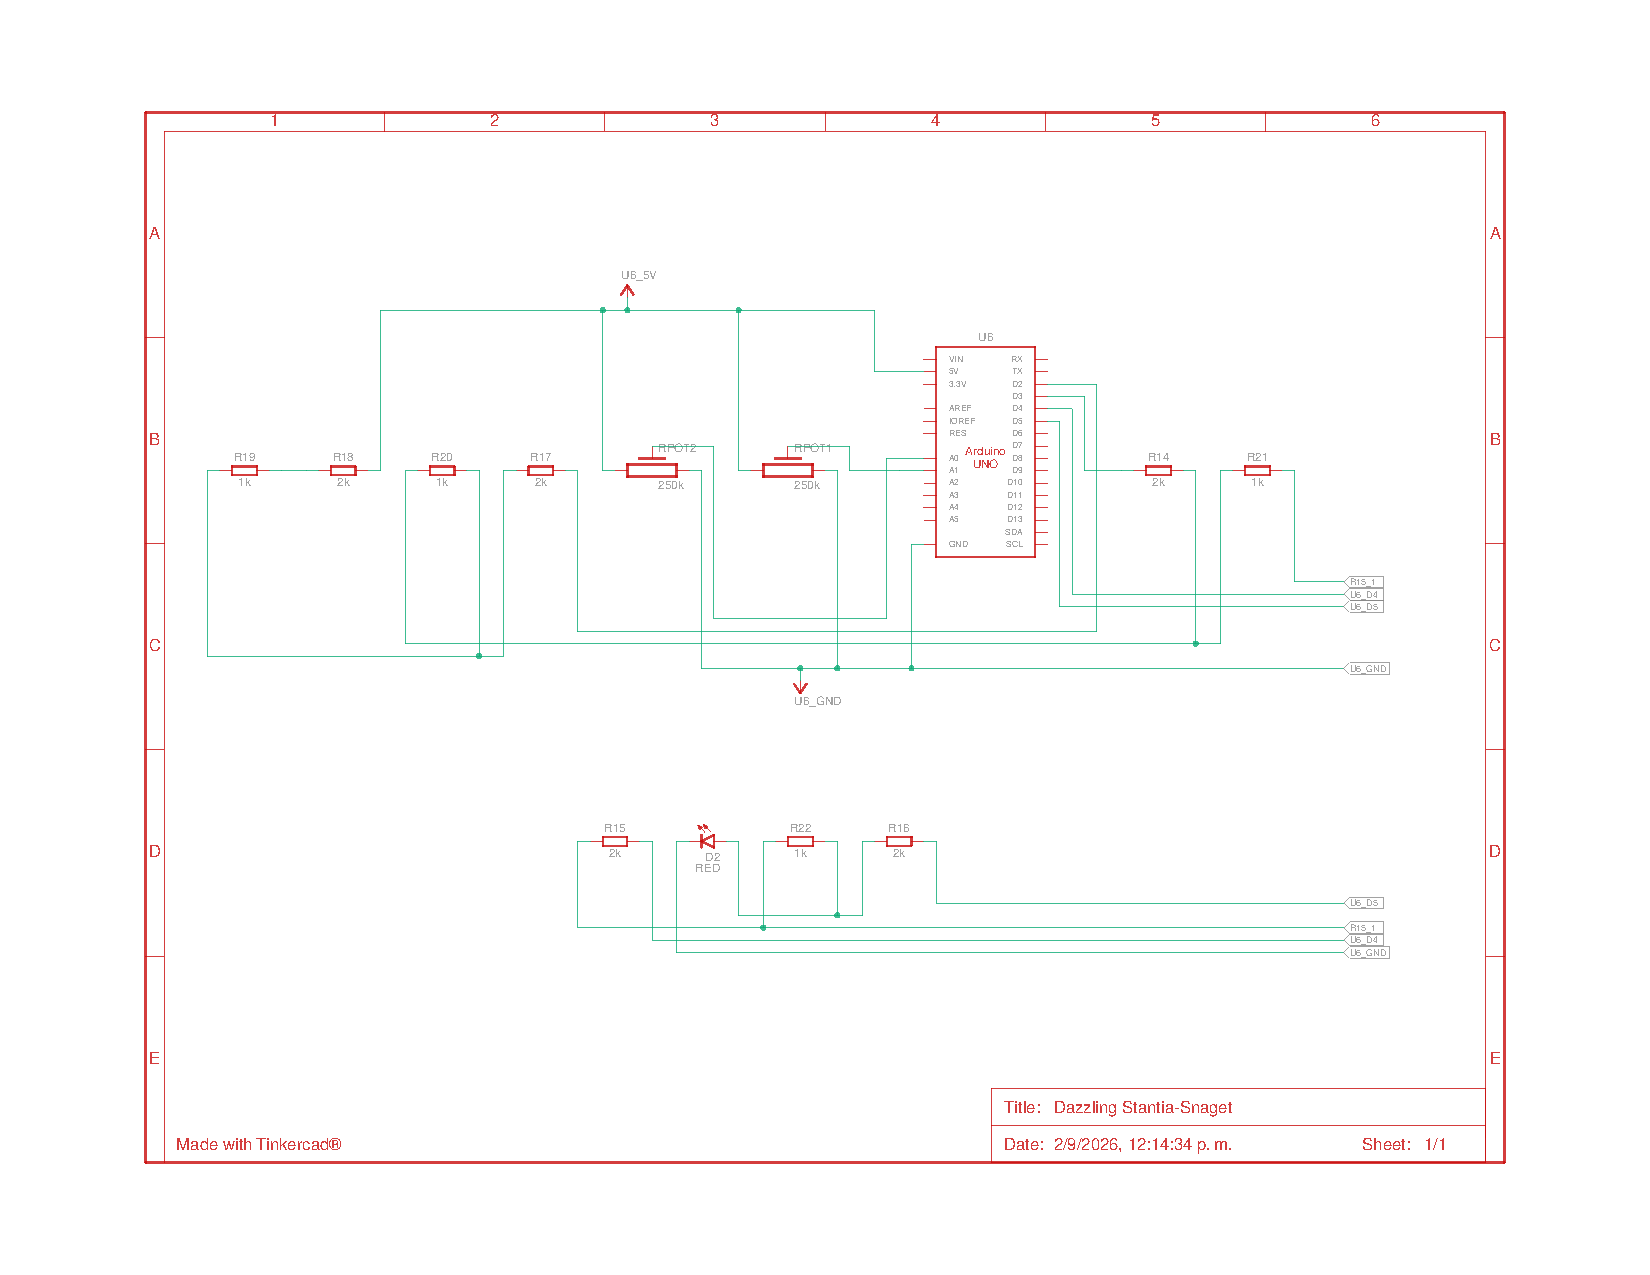
\includegraphics[width=\linewidth]{esquematico.pdf}
  \caption[Esquemático del circuito]{Esquemático del circuito. El potenciómetro de
  A0 fija la amplitud de la señal y el de A1 su frecuencia; la escalera R-2R,
  formada por las resistencias de
  \qty{1}{\kilo\ohm} y \qty{2}{\kilo\ohm}, devuelve al mundo analógico la señal que
  calcula el programa. Exportado de Tinkercad.}
  \label{fig:esquematico}
\end{figure}

\begin{figure}[H]
  \centering
  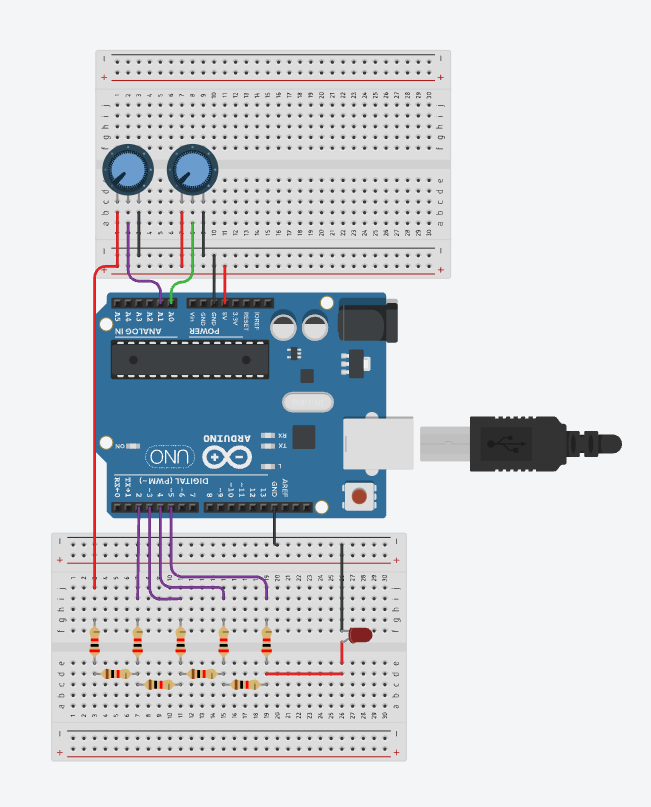
\includegraphics[width=0.62\linewidth]{montaje_protoboard.png}
  \caption[Montaje sobre protoboard]{Montaje sobre protoboard, que sirve de
  referencia para el cableado: los dos potenciómetros por un lado y la escalera
  R-2R con el LED por otro. La imagen los reparte en dos protoboards, pero todo el
  montaje cabe en una.}
  \label{fig:montaje}
\end{figure}

\FloatBarrier
%=======================================================================
\section{Desarrollo}
%=======================================================================

\subsection{El programa de partida}
Se entrega un programa que ya funciona y que genera una \textbf{señal senoidal}. Es el
modelo que va a reutilizar en la tarea, así que conviene entenderlo antes de tocarlo.

La idea es que \textbf{la señal se dibuja por puntos}. El programa parte cada ciclo en
\num{64} trozos y calcula qué valor le toca a cada uno. Después redondea ese valor al
escalón más cercano de los \num{16} que tiene la escalera y lo saca por los pines D2 a
D5. Repitiendo eso muy rápido, en la salida aparece la onda.

Los dos potenciómetros mandan sobre esa onda:

\begin{itemize}
    \item \textbf{A0 cambia la altura} de la señal, es decir su amplitud: desde plana
          hasta ocupar todo el rango.
    \item \textbf{A1 cambia lo rápido que se repite}, es decir su frecuencia: entre
          \num{1} y \num{500} veces por segundo.
\end{itemize}

El programa manda además dos números al puerto serie: el valor \textbf{exacto} que
debería tener la señal y el valor \textbf{redondeado} que realmente sale por la
escalera. Ábralos con el \emph{Serial Plotter} del IDE y verá las dos curvas
superpuestas: lo que se separan es lo que la señal pierde al pasar por el DAC.

\noindent\textbf{Antes de programar nada}, cargue el programa tal como está y gire los
dos potenciómetros mirando el osciloscopio --- o el \emph{Serial Plotter}, si no tiene
el osciloscopio delante. Uno debe cambiar la altura de la onda; el otro, cuántas veces
se repite.

\subsection{Tarea: cuatro señales más}
El programa entregado solo sabe hacer una senoide. \textbf{Programe otras cuatro formas
de onda} sobre ese mismo esqueleto, cambiando únicamente el cálculo del valor de cada
muestra:

\begin{enumerate}[label=\textbf{\alph*)}, leftmargin=*, labelsep=0.6em]
    \item \textbf{Rampa} o diente de sierra: crece de forma constante durante todo el
          ciclo y cae de golpe al empezar el siguiente.
    \item \textbf{Cuadrada}: se mantiene en el valor máximo media parte del ciclo y en
          el mínimo la otra media.
    \item \textbf{Triangular}: sube de forma constante durante medio ciclo y baja de la
          misma manera durante el otro medio.
    \item \textbf{Senoidal rectificada} de onda completa: la senoide del programa, pero
          con la mitad negativa volteada hacia arriba.
\end{enumerate}

\noindent Las cuatro deben seguir respondiendo a los potenciómetros igual que la
senoide: \textbf{A0 cambia su altura y A1 lo rápido que se repite}.

\medskip
\noindent De \textbf{cada una} de las cuatro señales debe entregar una \textbf{captura
del Serial Plotter} en la que se vean a la vez las dos trazas, la ideal y la
cuantizada.

\noindent Al terminar, responda sobre lo que ha visto:

\begin{enumerate}[label=\textbf{\arabic*.}, leftmargin=*, labelsep=0.6em]
\needspace{7\baselineskip}\item De las cuatro señales, ¿en cuál se notan más los escalones del DAC y en cuál
menos? Explique por qué a partir de la forma de cada una.
\lineasresp{3}

\needspace{7\baselineskip}\item La señal cuadrada solo necesita dos valores distintos. ¿Qué ventaja tiene
entonces reconstruirla con un DAC de cuatro bits en lugar de con un solo pin digital?
\lineasresp{3}

\needspace{7\baselineskip}\item Suba la frecuencia con A1 hasta el máximo. ¿Consigue de verdad que la señal se
repita \num{500} veces por segundo? Tenga en cuenta que en cada punto el programa envía
además dos números por el puerto serie: calcule cuánto tarda eso y compárelo con lo que
debería durar un punto.
\lineasresp{3}
\end{enumerate}

\FloatBarrier

% =====================================================================
% PENDIENTE: V. Cuestionario y VI. Conclusiones. Faltan tambien los \puntos{n}
% de las secciones calificadas, que deben sumar 20: no se reparten hasta que
% esten escritas todas, o los numeros no cuadran.
%
% La seccion de Construccion que tienen las guias de Circuitos aqui no hace
% falta: el montaje son dos potenciometros y nueve resistencias sobre
% protoboard, y las figuras 1 y 2 de la seccion III ya lo resuelven.
% =====================================================================

\end{document}
